\documentclass{easychair}

% \usepackage{doc}
\usepackage{setspace}
\usepackage{verbatim}

%----Making things more compact
\newcommand{\smalltt}[1]{\small \texttt{#1}}
\newenvironment{packed_itemize}{
\vspace*{-0.2em}
\begin{itemize}
\setlength{\partopsep}{0pt}
\setlength{\itemsep}{1pt}
\setlength{\parskip}{0pt}
\setlength{\parsep}{0pt}
}{\end{itemize}}
\newenvironment{packed_enumerate}{
\vspace*{-0.2em}
\begin{enumerate}
\setlength{\partopsep}{0pt}
\setlength{\itemsep}{1pt}
\setlength{\parskip}{0pt}
\setlength{\parsep}{0pt}
}{\end{enumerate}}
% \renewcommand{\textfraction}{0.07}
% \renewcommand{\topfraction}{0.9}
% \renewcommand{\bottomfraction}{0.9}
% \renewcommand{\floatpagefraction}{0.66}
% \setlength{\floatsep}{2.0pt plus 2.0pt minus 2.0pt}
% \setlength{\textfloatsep}{5.0pt plus 2.0pt minus 0.0pt}

%----For Alex's proof stuff
\usepackage{amsmath,amssymb,amsthm}
\newtheorem*{lemma}{Lemma}
\newtheorem*{theorem}{Theorem}
\newcommand{\true}{{\mathit{true}}}
\newcommand{\false}{{\mathit{false}}}

\title{The New TPTP Format for \\ Tarskian and Kripke Interpretations}

\author{
  Geoff Sutcliffe\inst{1}
\and
  Alexander Steen\inst{2}
\and
  Pascal Fontaine\inst{3}
}

\institute{
  University of Miami,
  Miami, USA\\
  \email{geoff@cs.miami.edu,jam771@miami.edu}
\and
  University of Greifswald,
  Greifswald, Germany\\
  \email{alexander.steen@uni-greifswald.de}
\and
  University of Li{\`e}ge,
  Li{\`e}ge, Belgium\\
  \email{Pascal.Fontaine@uliege.be}
}

\authorrunning{Sutcliffe, Steen, Fontaine}
\titlerunning{TPTP World Interpretations}

\begin{document}
\maketitle

%--------------------------------------------------------------------------------------------------
\begin{abstract}
This paper describes a new format for representing Tarskian and Kripke interpretations.
%formulae in untyped and typed first-order logic, using the TPTP TF0 language.
\end{abstract}
%--------------------------------------------------------------------------------------------------
\section{Introduction}
\label{Introduction}

Historically, Automated Theorem Proving (ATP) has, as the name suggests, focused largely on the
task of proving theorems from axioms -- the derivation of conclusions that follow inevitably 
from known facts \cite{RV01-HAR}.
The axioms and conjecture to be proved (and hence become a theorem) are written in an 
appropriately expressive logic, and the proofs are often similarly written in logic \cite{SS+06}.
% In this work simply-typed first-order logic in the form of \cite{Wal83,Sch85,Coh87},
% whose expressive power is sufficient for a wide range of topics \cite{Sut17}, is used
In the last two decades the converse task of disproving conjectures, i.e., proving that a 
conjecture is not a theorem of the axioms, has become increasingly important.
This process depends on finding an {\em interpretation}, i.e., a structure that maps terms 
to domain elements and formulae to truth values.
An interpretation that maps a formula to {\em true} is a {\em model} of the formula.
A conjecture is disproved by finding an interpretation that is a model of the axioms, but 
is not a model of the conjecture, aka a {\em countermodel} for the conjecture.
A salient application area that harnesses this form of ATP is verification \cite{DKW08},
where a countermodel is used to pinpoint the reason why a proof obligation fails, and
correspondingly points to the location of the fault in the system being verified.
Other applications of model finding include checking the consistency of an axiomatization 
\cite{SS+17}, and finding a solution to a problem that is coded as a model finding problem 
\cite{Win82}.

The TPTP World \cite{Sut17} (\href{https://www.tptp.org}{\tt www.tptp.org}) is a well established 
infrastructure that supports research, development, and deployment of Automated Theorem Proving 
(ATP) systems.
Various parts of the TPTP World have been deployed in a range of applications,
in both academia and industry.
The TPTP World includes the TPTP problem library \cite{Sut09}, 
the TSTP solution library \cite{Sut10}, 
tools and services for processing ATP problems and solutions \cite{Sut10}, 
it supports the CADE ATP System Competition (CASC) \cite{Sut16}.
The TPTP language \cite{Sut23-IGPL} is one of the keys to the success of the TPTP World.
Originally the TPTP World supported only first-order clause normal form (CNF)
\cite{SS98-JAR}.
Over the years full first-order form (FOF)
\cite{Sut09}, 
typed first-order form (TFF)
\cite{SS+12,BP13-TFF1}, 
typed extended first-order form (TXF)
\cite{SK18}, 
typed higher-order form (THF)
\cite{SB10,KSR16}, 
and non-classical forms (NTF).
Most relevant to this work, the TPTP languages are used for writing ATP problems, 
derivations, and interpretations \cite{SS+06,Sut08-KEAPPA}.
Examples of problems are in Appendices~\ref{FOF_Finite.p}, \ref{TFF_Finite.p},
\ref{TFF_Infinite.p}, \ref{NTF_Finite-Finite-Global.p}, and \ref{NTF_Finite-Finite-Local.p}.
The problems will be discussed in the context of their associated models in 
Sections~\ref{NewTarskian} and~\ref{NewKripke}.

A TPTP format for interpretations with finite domains \cite{SS+06} was previously been defined, 
and has served the ATP community adequately for almost 20 years. 
The old format is output by several ATP systems, e.g., Paradox \cite{CS03}, FMDarwin \cite{BF+06}, 
Vampire \cite{KV13}.
The new format replaces the old format for finite interpretations \cite{SS+06}, which 
Recently the need for a format for interpretations with infinite domains, and for a format for 
Kripke interpretations \cite{Kri63} of formulae written in the NTF language \cite{SF+22}, 
led to the development of a new TPTP format for interpretations.
This work describes the new TPTP format for interpretations.
The underlying principle is unchanged: interpretations are represented as formulae.

\paragraph{Related Work:}
Section~\ref{TypesOfInterpretations} provides the landscape of different representations of
interpretations, and how models (interpretations that make particular formulae {\em true})
can be built.
The focus there is on Tarskian interpretations, but Kripke interpretations are also reviewed.
That provides the necessary background for the focus of this paper -- a concrete realization
of how interpretations are to be represented in the TPTP World.
There are other concrete representations in use:
The SMT-LIB standard \cite{BFT17} defines a format for model output, and commands to inspect 
models.  
SAT solvers generally output models as specified by the SAT competitions \cite{JL+12}, in a 
simple format similar to the DIMACS input format \cite{Bab93}.
Some individual model finding systems have defined their own formats for models, e.g., the 
output formats of Nitpick and Z3 \cite{dMB08}.
% +++
% Nikolaj says ...
% Z3 It produces models that define functions by expressions. For example a model of succ is 
% Succ(x) =X+ 1
% Works when domain is integer. Currently z3 does not implement infinite models for uninterpreted sorts. I would probably support infinite sorts by creating injection into an algebraic datatype and then support models that can be expressed over ADT.
% See also https://microsoft.github.io/z3guide/docs/logic/Quantifiers
% +++

This paper is organized as follows:
Section~\ref{TypesOfInterpretations} discusses the nature of interpretations, considering what is
needed from interpretations, and the various forms that interpretations can take.
Section~\ref{NewTarskian} defines the new format for Tarskian interpretations, and
Section~\ref{NewKripke} does the same for Kripke interpretations.
Section~\ref{Tools} reviews some TPTP World tools for examining and manipulating interpretations.
Section~\ref{Conclusion} concludes and discusses plans for future work.

%--------------------------------------------------------------------------------------------------
\section{Uses for Interpretations}
\label{UsesForInterpretations}

What do we Need?
\begin{itemize}
\item {\em Model existence}
      \begin{packed_itemize}
      \item Consistency of axiomatizations, to avoid CAX [ATP process]
      \item Use as a yes/no subroutine in more complex reasoning [Steen], including~\ldots
      \item Axiom selection \cite{SP07} NEED FROM LT
      \item Existence of bugs in verification, but frustrating [McCune]
      \end{packed_itemize}
      The model finder has to be trusted.
\item {\em Explicit models}
      \begin{packed_itemize}
      \item Identification of bugs in verification [Claessen]
      \item A solution to a problem encoded as a model finding problem [Claessen]
      \item Inspecting outcomes of student's experiments [Steen]
      \item Evaluating formulae wrt the model [Sutcliffe]
      \item Machine learning from models [~Barbosa]
      \item Improve model finders [~Barbosa]
      \end{packed_itemize}
      The models can be verified.
\item {\em Properties of explicit interpretations}
      \begin{packed_itemize}
      \item Verifiable [Zhang]
      \item Comprehensible for manual inspection, e.g., for Intel \cite{EK+10}
      \item Tractable evaluation of formulae [Sutcliffe]
      \end{packed_itemize}
      In the language of the input!
\end{itemize}

This provides the basis for verification of models, as explained in Section~\ref{Verification}.

%--------------------------------------------------------------------------------------------------
\subsection{Model Verification}
\label{Verification}

ATP systems are complex pieces of software, implementing complex calculi, with the end goal
being a sound implementation of a sound inference system whose output correctly corroborates the
result obtained.
The reality is that the complexity leads to incorrectness, and as such verification of ATP systems'
outputs is necessary. 
For theorem proving this means verifying the proof output \cite{Sut06}, and for model finding 
this means verifying the model output.
In the context of this work the model verification applies to the type declarations and 
the interpretation formula that represent the model found by the ATP system, and
has (at least) the following aspects:
\begin{packed_enumerate}
\item Are the type declarations and interpretation formula syntactically well-formed 
      and semantically well-typed?
\item Is the interpretation formula satisfiable?
\item Does the interpretation formula correctly represent the interpretation found by the 
      ATP system?
\item Is the interpretation represented by the interpretation formula a model for the given 
      formulae?
\end{packed_enumerate}
\noindent
These questions are answered as follows:
\begin{enumerate}
\item This can be confirmed using standard parsing and type checking tools, e.g., \cite{VS06,HR15}.
\item This can be empirically confirmed using a trusted model finder (in the same way the GDV 
      derivation verifier \cite{Sut06} uses the Otter system \cite{McC03-Otter} as a trusted 
      theorem prover).
      Confirming that the interpretation formula is satisfiable is almost certainly much 
      easier than finding the model itself, so the system used to check the satisfiability can 
      be weaker and more trusted than the system that found the model.
\item This cannot be confirmed, as that representation is internal to the ATP system that found
      the model.
\item In this work a ``semantic'' approach is taken, in which the given formulae $\Phi$ are proved 
      from the interpretation formula $\varphi$ using a trusted theorem prover; $\varphi$ is 
      supplied as an axiom, and $\Phi$ as the conjecture to be proved.
      This approach relies on the proof of soundness below, which shows that if $\Phi$ can be 
      proved from $\varphi$ (written $\varphi \models \Phi$), then the interpretation $I$ 
      represented by $\varphi$ is a model of $\Phi$.

      An implementation is available online as the AGMV tool in the SystemOnTSTP \cite{Sut07-CSR} 
      web interface {\smalltt{\url{https://www.tptp.org/cgi-bin/SystemOnTSTP}}}.
      The tool input is the concatenation of the problem and the interpretation.
      Appendix~\ref{FOF_Finite.s.p} shows the verification problem for the problem in 
      Appendix~\ref{FOF_Finite.p} and its finite model in Appendix~\ref{FOF_Finite.s}.
      Appendix~\ref{TFF_Finite.s.p} shows the verification problem for the problem in 
      Appendix~\ref{TFF_Finite.p} and its finite model in Appendix~\ref{TFF_Finite.s}.
      Appendix~\ref{TFF_Integer.s.p} shows the verification problem for the problem in 
      Appendix~\ref{TFF_Infinite.p} and its integer model in Appendix~\ref{TFF_Integer.s}.
      Appendix~\ref{TFF_Peano.s.p} shows the verification problem for the problem in 
      Appendix~\ref{TFF_Infinite.p} and its infinite term model in Appendix~\ref{TFF_Peano.s}.
\end{enumerate}

%--------------------------------------------------------------------------------------------------
\section{Types of Interpretations}
\label{TypesOfInterpretations}

A Tarskian-style interpretation \cite{TV56} of formulae in first-order logic consists of a 
non-empty domain of unequal elements for each type used in the formulae (just one domain for 
untyped logic), and interpretations of the function and predicate symbols with respect to the 
domains \cite{Hun96,Gal15}.
An overview of some ways of building and representing Tarskian interpretations is provided 
by \cite{CLP04}.
$I \vdash \Phi$ means the interpretation $I$ is a model of the formula $\Phi$.
An interpretation can normally interpret all expressions that can be written in the language of 
the formulae, but in some circumstances an interpretation can interpret only (at least) the given 
formulae, e.g., \cite{BSW23}; such an interpretation is a {\em partial interpretation}.

Three types of Tarskian interpretations are clear (and more might exist):
\begin{itemize}
\item {\em Finite interpretations} have only finite domains.
      The domain and symbol mappings can be be explcitly enumerated.
      There are several ATP systems that produce finite interpretations, e.g., Paradox,
      FMDarwin, and Vampire.
      Finite interpretations are typically verifiable, comprehensible, and tractable.
\item {\em Infinite interpretations} have one or more infinite domains.
      Infinite domains can be explicitly generated (e.g., terms representing Peano numbers), or 
      implicitly specified (e.g., some set of algebraic numbers, such as the integers).
      There are several ATP systems that produce finite interpretations, e.g., 
      cvc5 \cite{BB+22-cvc5}, Z3.
      Infinite interpretations are verifiable, but might not be comprehensible, and are often
      intractable.
\item {\em Herbrand interpretations} \cite{Her30} have the Herbrand universe as the domain, 
      the mapping for non-boolean symbols (functions) is the ``identity'', and the mapping
      for boolean symbols (predicates) is from the Herbrand base to $\{true,false\}$.

      Every set of formulae induces its set of Herbrand models.
      A set of formulae might not be intended to represent it's models, e.g., the input to 
      an ATP system. 
      In the ATP context a set of formulae is often intended to at least confirm the existence
      of Herbrand models.
      Such sets can be the result from model preserving transformations done by an ATP on its 
      input, or generated by an ATP system with the explicit intention of representing Herbrand 
      interpretations.
      \begin{packed_itemize}
      \item {\em Saturations} \cite{BG+01} are a fixed point for a set of clauses at which further 
            application of a complete inference system does not generate any new clauses.
            This approach is adopted in saturation-based ATP systems such as E \cite{SCV19},
            Prover9 \cite{McC-Prover9-URL}, Vampire, and Zipperposition \cite{VB+21}.
            While the domain of a saturation is known to be the Herbrand Universe, there is no 
            explicit symbol interpretation that can be used constructively by users.
            Saturations are verifiable, incomprehensible, and often intractable.
      \item {\em Formulae} that are intended to represent Herbrand interpretations include
            a disjunction of implicit generalisations (DIGs) \cite{LM87}, and predicate
            definitions over the term algebra \cite{SK12}.
            iProver \cite{Kor08,SK12} is an ATP system that output the latter format.
            Formulae as Herbrand interpretations are verifiable, and they can be comprehensible 
            and tractable.
      \end{packed_itemize}
\item {\em Kripke interpretations} \cite{Kri63} add a layer of {\em worlds} over Tarskian
      interpretations.
      There can be a finite or infinite number of worlds.
      There is an {\em accessibility relation} between the worlds, which can be subject to the
      requirements of the logic being used, e.g., for modal logic {\bf M} the accessibility 
      relation must be reflexive, i.e., every world can access itself.
      Within each world there is a Tarskian interpretation, and there can be some interaction
      between the worlds' interpretations if the terms designate globally MORE TO BE SAID.
      The verifiability, comprehensibility, and tractablity of Kripke interpretations varies
      between individual cases.
\end{itemize}

The notions of interpretations, models, partial interpretations, finite interpretations,
Herbrand interpretations, etc., are captured in the SZS ontologies \cite{Sut08-KEAPPA}, as
updated at 
\href{https://www.tptp.org/cgi-bin/SeeTPTP?Category=Documents\&File=SZSOntology}{\tt www.tptp.org}
\href{https://www.tptp.org/cgi-bin/SeeTPTP?Category=Documents\&File=SZSOntology}{\tt /cgi-bin/SeeTPTP?Category=Documents\&File=SZSOntology}.
For this work the otology was extended with a new value {\em Model Preserving} (MPR), defined
as ``Some interpretations are models of Ax, and
  all models of Ax are extended to a model of C, and
  all models of C are an extension of a model of Ax
  (which means that all models of C are models of Ax)''.
This is used for ATP transformations of satisfiable sets of formulae in which the models
of the set are unchanged, or changed only by adding new domain elements or mappings such
that they still model the original formulae.
Examples of such transformations are adding logical consequence of the set into the set, and
Skolemization.

Ways to make finite interpretations:
\begin{packed_itemize}
\item Reduction to Function-Free Clause Logic \cite{CS03,McC03-MACE4-TR,BF+09}
\end{packed_itemize}

Ways to make infinite non-Herbrand interpretations:
\begin{packed_itemize}
\item cvc5
\end{packed_itemize}

Ways to make Herbrand interpretations:
\begin{packed_itemize}
\item Tableaux. as long as you use a proof confluent calculus, it is normally possible to 
      construct a model from a saturated branch \cite{Hah01}.
\item Hyper-tableaux. \cite{BFN96,Bau98,BFP07}
\item Ordered Semantic Hyper-linking \cite{PZ00} NEED TO READ
\item SGGS \cite{BP16}
\item Proving Infinite Satisfiability \cite{BB13}
\item Model Evolution with Equality \cite{BT03,BFT04,BT05,BPT11}
\item EQMC \cite{CP00,Pel03-EQMC}
\item Saturation \cite{Pel03-JSC}
\item RAMC \cite{CZ92,CP95,CP95-TAB}
\end{packed_itemize}

\begin{figure}[htbp]
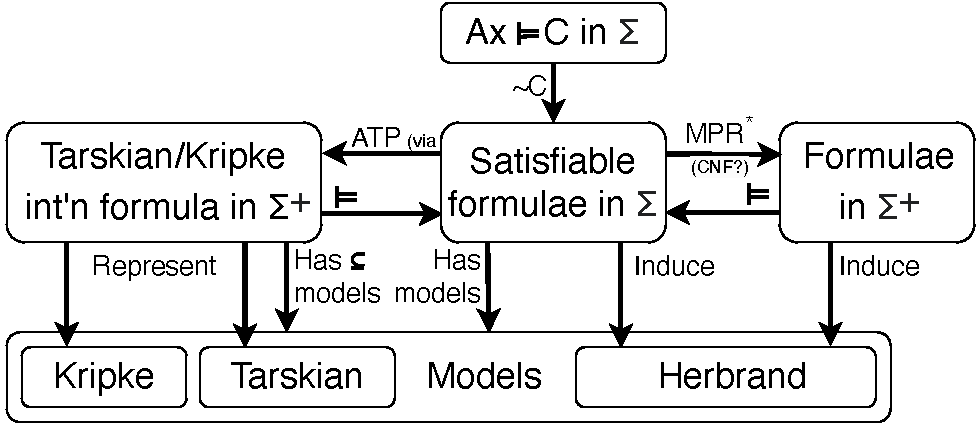
\includegraphics[width=\textwidth]{ModelLandscape.pdf}
\caption{The Landscape of Classical Model Building}
\label{ModelLandscape}
\end{figure}

%--------------------------------------------------------------------------------------------------
\section{The New Format for Tarskian Interpretations}
\label{NewTarskian}

As noted in Section~\ref{Introduction}, a TPTP format for interpretations with finite domains 
has previously been defined, and was been adopted by some ATP systems.

The new format uses an {\em interpretation formula}. 
Examples of single interpretation formulae are in Appendices~\ref{FOF_Finite.s},
\ref{TFF_Finite.s}, \ref{TFF_Integer.s}, and~\ref{TFF_Peano.s}, illustrating the components 
described next. 
(Interpretations split over multiple interpretation formulae, as in 
Appendices~\ref{FOF_Finite_Medium.s}, \ref{TFF_Finite_Fine.s}, and~\ref{TFF_Finite_Compact.s},
are explained below.)

An interpretation formula is a conjunction of components:
\begin{packed_itemize}
\item Domain specifications for each of the types in the problem formulae.
      Each domain specification is a 
      conjunction of:
      for each type a {\em type-promotion} function that converts domain elements to terms is
      used to keep the interpretation formula well-typed; 
      \begin{packed_itemize}
      \item the domain type, by a formula that makes the type-promotion function a surjection 
            (unless it is unnecessary because the type is defined and is the same as the type in 
            the given formulae, e.g., both are {\smalltt{\$int}});
      \item the domain elements (unless implicit from their defined type): if the domain is
            finite this is a universally quantified disjunction of equalities whose right-hand 
            sides are the terms; if the domain is infinite an existentially quantified formula 
            that captures an infinite disjunction of equalities is used, e.g., for terms 
            representing Peano numbers as the domain elements:\\
            \hspace*{0.5cm}$\forall I{:}peano\;((I = zero) \vee \exists P{:}peano\;(I = s(P)))$;
%            \smalltt{! [I: peano] : ( I = zero | ? [P: peano] : I = s(P) )};
      \item specification of the distinctness of the domain elements (unless implicit from their
            defined type);
      \item a formula making the type-promotion function an injection,
            % (unless the type of the domain is the same as the type in the formula), 
            which together with the surjectivity makes it a bijection.
      \end{packed_itemize}
\item interpretation of the function symbols, as equalities whose left-hand sides are 
      formed from symbols applied to type-promoted domain elements, and whose right-hand sides 
      are type-promoted domain elements;
\item interpretation of the predicate symbols, as literals formed from symbols applied
      to type-promoted domain elements; positive literals are {\em true} and negative literals 
      are {\em false}.
\end{packed_itemize}
The interpretation formula is preceded by the necessary type declarations:
\begin{packed_itemize}
\item the types in the given formulae (except defined types, e.g., {\smalltt{\$int}});
\item the types of the domains (except defined types);
\item the types of type-promotion functions;
\item the types of the domain elements.
\end{packed_itemize}
% \vspace*{-0.4em}
This representation is also directly usable for untyped first-order logic, where all terms in 
the given formulae and the interpretation formula are of the same type – ``individuals''. 
This obviates the need for type considerations, in particular type-promotion functions are not 
needed.

Appendix~\ref{TFF_Finite.s} shows a TF0 interpretation with finite domains -- it is a 
countermodel for the problem in Appendix~\ref{TFF_Finite.p}.
The comments show which parts of the formula specify what aspects of the interpretation.
Appendix~\ref{TFF_Integer.s} shows a TF0 interpretation with an integer domain -- it 
is a model for the problem in Appendix~\ref{TFF_Infinite.p}.
Note that in Appendix~\ref{TFF_Integer.s}:
the defined type {\smalltt{\$int}} is the domain type for the formula type 
{\smalltt{person}}, so that there is no specification of the domain elements and their 
distinctness;
universal quantification is used for the interpretation of function and predicate
symbols for an infinite number of argument tuples;
the interpretations of function and predicate symbols is not given for argument 
tuples with negative integers, i.e., this is an example of a partial interpretation.
Appendix~\ref{TFF_Peano.s} shows a TF0 interpretation with an infinite term domain -- it 
is a model for the problem in Appendix~\ref{TFF_Infinite.p}.

%--------------------------------------------------------------------------------------------------
\section{The New Format for Kripke Interpretations}
\label{NewKripke}
 
The new format uses an {\em interpretation formula}. 
Examples of single interpretation formulae are in Appendices~\ref{NTF_Finite-Finite-Global.s}
and~\ref{NTF_Finite-Finite-Local.s}, illustrating the components 
described next. 
(Interpretations split over multiple interpretation formulae, as in 
Appendices~\ref{NTF_Finite-Finite-Global_Medium.s}, \ref{NTF_Finite-Finite-Global_Fine.s},
and~\ref{NTF_Finite-Finite-Global_Compact.s}, are explained below.)

%--------------------------------------------------------------------------------------------------
\section{Tools for Interpretations}
\label{Tools}

%--------------------------------------------------------------------------------------------------
\section{Conclusion}
\label{Conclusion}

This paper 

This work is being extended 

%--------------------------------------------------------------------------------------------------
\bibliographystyle{plain}
\bibliography{Bibliography.bib}
%--------------------------------------------------------------------------------------------------
\newpage
\appendix

All these listings are available from
\href{https://github.com/GeoffsPapers/InterpretationFormat}{github.com/GeoffsPapers/InterpretationFormat}.

\section{FOF Listings}
\label{FOFListings}

\subsection{A FOF Problem with a Finite Countermodel}
\label{FOF_Finite.p}
\begin{small}
\verbatiminput{FOF_Finite.p}
\end{small}

\newpage
\subsection{A FOF Interpretation with a Finite Domain}
\label{FOF_Finite.s}
\begin{small}
\verbatiminput{FOF_Finite.s}
\end{small}

\newpage
\subsection{A FOF Interpretation with a Finite Domain, Medium Grained}
\label{FOF_Finite_Medium.s}
\begin{small}
\verbatiminput{FOF_Finite_Medium.s}
\end{small}

\newpage
\subsection{A FOF Interpretation with a Finite Domain, Verification Problem}
\label{FOF_Finite.s.p}
\begin{small}
\verbatiminput{FOF_Finite.s.p}
\end{small}

%--------------------------------------------------------------------------------------------------
\newpage
\section{TF0 Listings}
\label{TF0Listings}

\subsection{A TF0 Problem with a Finite Countermodel}
\label{TFF_Finite.p}
\begin{small}
\verbatiminput{TFF_Finite.p}
\end{small}

\newpage
\subsection{A TF0 Interpretation with a Finite Domain}
\label{TFF_Finite.s}
\begin{small}
\verbatiminput{TFF_Finite.s}
\end{small}

\newpage
\subsection{A TF0 Interpretation with a Finite Domain, Medium Grained}
\label{TFF_Finite_Medium.s}
\begin{small}
\verbatiminput{TFF_Finite_Medium.s}
\end{small}

\newpage
\subsection{A TF0 Interpretation with a Finite Domain, Fine Grained}
\label{TFF_Finite_Fine.s}
\begin{small}
\verbatiminput{TFF_Finite_Fine.s}
\end{small}

\newpage
\subsection{A TF0 Interpretation with a Finite Domain, Compacted}
\label{TFF_Finite_Compact.s}
\begin{small}
\verbatiminput{TFF_Finite_Compact.s}
\end{small}

\newpage
\subsection{A TF0 Problem with an Infinite Model}
\label{TFF_Infinite.p}
\begin{small}
\verbatiminput{TFF_Infinite.p}
\end{small}

\newpage
\subsection{A TF0 Interpretation with an Integer Domain}
\label{TFF_Integer.s}
\begin{small}
\verbatiminput{TFF_Integer.s}
\end{small}

\newpage
\subsection{A TF0 Interpretation with an Infinite Term Domain}
\label{TFF_Peano.s}
\begin{small}
\verbatiminput{TFF_Peano.s}
\end{small}

\newpage
\subsection{A TF0 Interpretation with a Finite Domain, Verification Problem}
\label{TFF_Finite.s.p}
\begin{small}
\verbatiminput{TFF_Finite.s.p}
\end{small}

\newpage
\subsection{A TF0 Interpretation with an Integer Domain, Verification Problem}
\label{TFF_Integer.s.p}
\begin{small}
\verbatiminput{TFF_Integer.s.p}
\end{small}

\newpage
\subsection{A TF0 Interpretation with an Infinite Term Domain, Verification Problem}
\label{TFF_Peano.s.p}
\begin{small}
\verbatiminput{TFF_Peano.s.p}
\end{small}

%--------------------------------------------------------------------------------------------------
\newpage
\section{NXF Listings}
\label{NXFListings}

\subsection{A NXF Problem with Global Axioms, with a Finite-Finite Countermodel}
\label{NTF_Finite-Finite-Global.p}
\begin{small}
\verbatiminput{NTF_Finite-Finite-Global.p}
\end{small}

\newpage
\subsection{A NXF Interpretation for Global Axioms, with Finite Worlds with Finite Domains}
\label{NTF_Finite-Finite-Global.s}
\begin{small}
\verbatiminput{NTF_Finite-Finite-Global.s}
\end{small}

\newpage
\subsection{A NXF Interpretation for Global Axioms, with Finite Worlds with Finite Domains, Medium Grained}
\label{NTF_Finite-Finite-Global_Medium.s}
\begin{small}
\verbatiminput{NTF_Finite-Finite-Global_Medium.s}
\end{small}

\newpage
\subsection{A NXF Interpretation for Global Axioms, with Finite Worlds with Finite Domains, Fine Grained}
\label{NTF_Finite-Finite-Global_Fine.s}
\begin{small}
\verbatiminput{NTF_Finite-Finite-Global_Fine.s}
\end{small}

\newpage
\subsection{A NXF Interpretation for Global Axioms, with Finite Worlds with Finite Domains, Compacted}
\label{NTF_Finite-Finite-Global_Compact.s}
\begin{small}
\verbatiminput{NTF_Finite-Finite-Global_Compact.s}
\end{small}

\newpage
\subsection{A NXF Problem with Global and Local Axioms, with a Finite-Finite Countermodel}
\label{NTF_Finite-Finite-Local.p}
\begin{small}
\verbatiminput{NTF_Finite-Finite-Local.p}
\end{small}

\newpage
\subsection{A NXF Interpretation for Global and Local Axioms, with Finite Worlds with Finite Domains}
\label{NTF_Finite-Finite-Local.s}
\begin{small}
\verbatiminput{NTF_Finite-Finite-Local.s}
\end{small}

\newpage
\subsection{A NXF Interpretation for Global Axioms, with Finite Worlds with Finite Domains, Verification Problem}
\label{NTF_Finite-Finite-Global.s.p}
\begin{small}
\verbatiminput{NTF_Finite-Finite-Global.s.p}
\end{small}

\newpage
\subsection{A NXF Interpretation for Global and Local Axioms, with Finite Worlds with Finite Domains, Verification Problem}
\label{NTF_Finite-Finite-Local.s.p}
\begin{small}
\verbatiminput{NTF_Finite-Finite-Local.s.p}
\end{small}

%--------------------------------------------------------------------------------------------------
\end{document}
%--------------------------------------------------------------------------------------------------
